\documentclass[11pt,a4paper]{article}
\usepackage[utf8]{inputenc}
\usepackage[T1]{fontenc}
\usepackage[brazil]{babel}
\usepackage{lmodern}
\usepackage{amsmath,amssymb,bm}
\usepackage{graphicx,booktabs,float,geometry,url,array,xcolor,caption}
\usepackage[hidelinks]{hyperref}
\geometry{margin=2.2cm}
\captionsetup{font=small}
\emergencystretch=2em
\providecommand{\versao}{sem versão}
% gerado por gera_dados.py; nao edite
\newcommand{\fsZero}{1{,}498}
\newcommand{\fsSeis}{1{,}472}
\newcommand{\fsDoze}{1{,}230}
\newcommand{\fsDezoito}{1{,}057}
\newcommand{\fsVquatro}{0{,}367}
\newcommand{\frenteSeis}{0{,}65}
\newcommand{\frenteDoze}{1{,}25}
\newcommand{\frenteDezoito}{1{,}85}
\newcommand{\tPassagem}{20{,}24}
\newcommand{\zcDoze}{1{,}075}
\newcommand{\zcDezoito}{1{,}675}
\newcommand{\kstarDezoito}{8{,}29}
\newcommand{\limDezoitoA}{0{,}000}
\newcommand{\limDezoitoB}{0{,}002}
\newcommand{\limDezoitoC}{0{,}006}
\newcommand{\kstarVinte}{2{,}66}
\newcommand{\limVinteA}{0{,}011}
\newcommand{\limVinteB}{0{,}056}
\newcommand{\limVinteC}{0{,}074}
\newcommand{\kstarVquatro}{0{,}836}
\newcommand{\limVquatroA}{0{,}557}
\newcommand{\limVquatroB}{0{,}420}
\newcommand{\limVquatroC}{0{,}353}
\newcommand{\mcDezesseisA}{0{,}524}
\newcommand{\mcDezesseisDezoitoA}{0{,}0000}
\newcommand{\mcDezesseisB}{0{,}385}
\newcommand{\mcDezesseisDezoitoB}{0{,}0020}
\newcommand{\mcDezesseisC}{0{,}321}
\newcommand{\mcDezesseisDezoitoC}{0{,}0054}
\newcommand{\difVqMin}{1{,}0}
\newcommand{\difVqMax}{6{,}4}
\newcommand{\difDzMin}{2{,}4}
\newcommand{\difDzMax}{11{,}3}
\newcommand{\zPyMax}{0{,}67}
\newcommand{\difPyMax}{0{,}32}
\newcommand{\tEqMin}{18{,}6}
\newcommand{\tEqMax}{20{,}5}
\newcommand{\nTeqSem}{0}
\newcommand{\pfBaseDz}{1{,}54}
\newcommand{\pfBaseVq}{37{,}1}
\newcommand{\pfBaseVqLo}{35{,}8}
\newcommand{\pfBaseVqHi}{38{,}4}
\newcommand{\pfBaseDzLo}{1{,}23}
\newcommand{\pfBaseDzHi}{1{,}92}
\newcommand{\pfPyBaseDz}{1{,}45}
\newcommand{\pfPyBaseDzSE}{0{,}05}
\newcommand{\pfPyBaseVq}{36{,}9}
\newcommand{\pfPyCincoDz}{1{,}48}
\newcommand{\pfPyCincoVq}{37{,}14}
\newcommand{\pfBaseDoze}{0{,}00}
\newcommand{\pfDozeMax}{0{,}64}
\newcommand{\baseDoze}{0{,}391}
\newcommand{\baseDezoito}{0{,}126}
\newcommand{\baseVq}{0{,}403}
\newcommand{\medDoze}{1{,}075}
\newcommand{\medDezoito}{1{,}350}
\newcommand{\medVq}{1{,}675}
\newcommand{\fsMedia}{0{,}882}
\newcommand{\fsDp}{0{,}397}
\newcommand{\fsMin}{0{,}3669}
\newcommand{\fsMax}{1{,}470}
\newcommand{\fsPico}{0{,}355}
\newcommand{\epsN}{5\,000}
\newcommand{\epsParou}{1\,506}
\newcommand{\epsParouPct}{30}
\newcommand{\epsCens}{1\,475}
\newcommand{\epsLimLo}{29{,}2}
\newcommand{\epsLimHi}{58{,}7}
\newcommand{\lsRec}{1{,}81}
\newcommand{\lsCvRec}{1{,}65}
\newcommand{\lsAnRec}{4{,}0}
\newcommand{\lsRecCem}{1{,}73}
\newcommand{\lsCvRecCem}{1{,}47}
\newcommand{\lsAnRecCem}{4{,}0}
\newcommand{\lsTdez}{1{,}68}
\newcommand{\lsCvTdez}{1{,}03}
\newcommand{\lsAnTdez}{3{,}9}
\newcommand{\lsTcinco}{1{,}71}
\newcommand{\lsCvTcinco}{1{,}09}
\newcommand{\lsAnTcinco}{3{,}8}
\newcommand{\lsEst}{2{,}18}
\newcommand{\lsCvEst}{1{,}22}
\newcommand{\lsAnEst}{3{,}8}
\newcommand{\lsPqui}{1{,}82}
\newcommand{\lsCvPqui}{4{,}10}
\newcommand{\lsAnPqui}{5{,}0}
\newcommand{\lsVq}{35{,}75}
\newcommand{\lsCvVq}{0{,}33}
\newcommand{\lsAnVq}{7{,}9}
\newcommand{\lsVqC}{34{,}82}
\newcommand{\lsCvVqC}{0{,}33}
\newcommand{\lsAnVqC}{9{,}1}
\newcommand{\lsPool}{1{,}83}
\newcommand{\lsPoolSE}{0{,}15}
\newcommand{\zPool}{2{,}5}
\newcommand{\dfsRaiz}{2{,}7}
\newcommand{\dfsRaizSE}{0{,}4}
\newcommand{\deslocRaiz}{0{,}11}
\newcommand{\deslocTres}{0{,}12}
\newcommand{\deslocQuatro}{0{,}16}
\newcommand{\pyCorr}{1{,}56}
\newcommand{\zPoolCorr}{1{,}7}
\newcommand{\zVq}{\ensuremath{-}0{,}76}
\newcommand{\zVqC}{\ensuremath{-}1{,}30}
\newcommand{\nRaizes}{16}

\newcommand{\lado}[4]{% figura de Cho (#1, largura #2) ao lado da nossa (#3, largura #4)
  \begin{minipage}[c]{#2\linewidth}\centering\includegraphics[width=\linewidth]{#1}\\[2pt]{\footnotesize Cho (2014)}\end{minipage}\hfill
  \begin{minipage}[c]{#4\linewidth}\centering\includegraphics[width=\linewidth]{#3}\\[2pt]{\footnotesize este trabalho}\end{minipage}}
\title{Cho (2014): a coluna 1D de talude infinito sob chuva\\ as figuras do artigo reproduzidas com o NeoPZ}
\author{Diogo Cecílio}
\date{24/11/2026 --- versão \versao}
\begin{document}
\maketitle
\begin{abstract}
Cho~\cite{cho2014} estuda uma coluna de 2~m de solo residual sobre rocha, num talude infinito de $40^\circ$, sob chuva
igual ao $k_s$ médio por 24~h, com $k_s$ lognormal em campo 1D. Refizemos todas as figuras de resultado do artigo (Figs.~3 e
5 a 10) com o \texttt{SlopeRainColumn} do NeoPZ: 15 casos de 5000 realizações no fermi, uma referência independente em
Python e os estudos de malha, esquema e $\varepsilon$. \textbf{Reproduz:} o determinístico (Fig.~3: FS mínimo
\fsZero/\fsSeis/\fsDoze/\fsDezoito/\fsVquatro{} em 0/6/12/18/24~h, dentro das faixas lidas); o limite de variável
aleatória ($l_v \to \infty$), que fecha os valores de Cho em 24~h; e, em 24~h, todas as tendências da Fig.~10, com a
$P_f$ de \difVqMin{} a \difVqMax{} pontos abaixo da de Cho (caso base: \pfBaseVq\,\% contra 43,4\,\%).
\textbf{Não reproduz:} os valores de 18~h. Ficamos \difDzMin{} a \difDzMax{} pontos abaixo, e os de Cho com $l_v$ grande
são incompatíveis com o próprio modelo do artigo: numa coluna homogênea a falha em 18~h exige $k_s > \kstarDezoito\,q$, o
que dá no máximo $0{,}6\,\%$, contra 5 a 11\,\% na Fig.~10a. \textbf{Os métodos conferem:} NeoPZ e Python coincidem nos 15
casos ($|z| \le \zPyMax$); a malha (ny 200), o elemento (tri) e a massa não mudam a $P_f$; e o line sampling concorda
com o MC, com um excesso em 18~h que a diferença de FS C++ $-$ Python nas raízes ($\approx -0{,}003$) explica.
\end{abstract}
\tableofcontents

\section{O que foi rodado}\label{sec:rodado}
\begin{itemize}
  \item \textbf{O problema~\cite{cho2014}:} coluna vertical de $H = 2$~m sobre rocha impermeável, talude infinito com
    $\beta = 40^\circ$, sucção inicial de 20~kPa, chuva de $q = 3\times10^{-6}$~m/s (10,8~mm/h, igual ao $k_s$ médio)
    por 24~h sem lâmina (o excesso escorre). Van Genuchten--Mualem com $\theta_s = 0{,}358$, $\theta_r = 3{,}58\times10^{-4}$,
    $\alpha = 0{,}149$~kPa$^{-1}$, $n = 1{,}289$. FS de Lu--Godt com $W = \int (\gamma_d + \theta\gamma_w)\,dz$, $c' = 5$~kPa,
    $\varphi' = 32^\circ$, $\gamma_d = 16$~kN/m$^3$; o FS mínimo é o menor nos nós da coluna, e a profundidade crítica
    $z_{crit}$, a desse nó.
  \item \textbf{O campo:} $k_s$ lognormal de média $q$ e $CoV = 0{,}5$, 1,0 e 1,5, núcleo $\exp(-|\Delta z|/l_v)$ com
    $l_v = 0{,}5$, 2, 4, 8 e 16~m (sem fator 2, como em Cho: a Fig.~4 confirma), base de Nyström no segmento com
    $M = 100$ termos (variância retida 0,992 com $l_v = 0{,}5$).
  \item \textbf{O modelo NeoPZ} (\texttt{SlopeRainColumn}): faixa de 0,025~m com 80 quadriláteros (massa consistente),
    $\Delta t = 0{,}1$~h, Newton \texttt{1e-6,80,1}, $k_r$ de Mualem tabelado com $\varepsilon = 10^{-3}$ (a correção do
    Newton com $n < 2$). A falha é a do artigo: FS mínimo $< 1$ no instante (aqui igual à de primeira passagem, porque a
    água só entra).
  \item \textbf{A campanha \texttt{cho2014} (fermi):} os 15 casos da Fig.~10 com 5000 realizações cada (o $N$ de Cho),
    todas pareadas (a realização $n$ tem os mesmos $\xi$ em todos os casos). Mais os estudos com 2000 realizações:
    ny 200 ($l_v$ 0,5 e 16), triângulos com massa concentrada e consistente; e $\varepsilon = 10^{-4}$ com 5000.
    Nenhuma realização dos 15 casos parou.
  \item \textbf{A referência em Python} (\texttt{coluna\_ref.py}, volumes finitos, $N = 200$, forma mista, o mesmo
    gerador): as mesmas 5000 realizações por caso, e 55\,000 no caso base.
  \item \textbf{O line sampling} no caso base em 18 e 24~h (Seção~\ref{sec:ls}).
\end{itemize}
Nenhuma simulação foi feita para este relatório: ele só lê resultados que já existiam
(Apêndice~\ref{sec:arquivos}). As figuras de Cho são recortes do PDF do artigo; os valores dele que entram nos nossos
gráficos vêm das notas de leitura~\cite{notas}: a Fig.~10 digitalizada ($\pm 0{,}002$) e as outras lidas a olho.

\section{Determinístico: a Fig.~3}\label{sec:det}
A Fig.~\ref{fig:det} põe os perfis do NeoPZ e do Python ao lado da Fig.~3 de Cho.
\begin{itemize}
  \item \textbf{O FS mínimo} vale \fsZero, \fsSeis, \fsDoze, \fsDezoito{} e \fsVquatro{} em 0, 6, 12, 18 e 24~h, contra
    $\approx 1{,}50$, 1,47, 1,25--1,27, 1,06 e 0,36--0,37 lidos de Cho. O de 12~h fica 0,02 abaixo da leitura; o de 24~h
    é o da coluna cheia e hidrostática, $0{,}5204/2 + 0{,}1067$.
  \item \textbf{A frente} está em \frenteSeis, \frenteDoze{} e \frenteDezoito~m em 6, 12 e 18~h (Cho: 0,60--0,65,
    1,15--1,25 e 1,75--1,85~m). O balanço de massa dá 0,59/1,19/1,78~m.
  \item \textbf{A profundidade crítica} sai da base (0 e 6~h) para logo atrás da frente (\zcDoze~m em 12~h e
    \zcDezoito~m em 18~h) e volta à base quando a frente chega à rocha, em $t = \tPassagem$~h. Aí o FS salta de
    $\approx 1{,}02$ para 0,37 em poucos minutos (Fig.~\ref{fig:det}c): com a base saturada e $u_w = 0$, o FS em 2~m é
    1,005, e 1,5~cm de água bastam para a falha.
  \item \textbf{O undershoot} da Fig.~3a (carga de $-2{,}10$ a $-2{,}15$~m logo à frente da frente) aparece com a massa
    consistente na malha de 0,05~m (ny 40); na malha de produção (0,025~m) ele quase some, sem mudar o FS (V3.3).
\end{itemize}
\begin{figure}[htbp]\centering
\lado{dados/cho_fig3.png}{0.33}{figs/fig3_det.pdf}{0.65}
\caption{A Fig.~3. (a) A carga de pressão (NeoPZ cheio, Python pontilhado; as barras largas são as frentes lidas de
Cho). (b) O FS ao longo da coluna (quadrados: o FS mínimo lido de Cho, na profundidade crítica). (c) O FS mínimo no
tempo (NeoPZ quad ny 80 a cada 3~h e em 16, 19 a 22~h; os quadrados pretos são as leituras de Cho).}
\label{fig:det}
\end{figure}

\section{Monte Carlo no caso base: as Figs.~5 a 8}\label{sec:base}
O caso base é $CoV = 0{,}5$ e $l_v = 0{,}5$~m. A Tabela~\ref{tab:alvos} resume os alvos.
\begin{itemize}
  \item \textbf{Fig.~5, a profundidade crítica (Fig.~\ref{fig:f5}):} a forma é a mesma. Em 12~h, uma moda em
    1,05--1,10~m e a barra da base; em 18~h, as superfícies se espalham de 0,8 a 1,95~m; em 24~h, a base domina. A fração na
    base sai \baseDoze, \baseDezoito{} e \baseVq{} em 12/18/24~h, contra 0,29/0,10/0,44: a nossa é 10 pontos maior em
    12~h, 3 pontos maior em 18~h e 4 pontos menor em 24~h. As nossas frentes ficam mais lentas nas colunas heterogêneas.
  \item \textbf{Fig.~6, o FS de 24~h (Fig.~\ref{fig:f6}):} a mesma distribuição bimodal: o pico da coluna cheia em
    0,36--0,39 (\fsPico{} contra 0,29), a moda de 1,05--1,08 e o pequeno pico em 1,45--1,48. A média é \fsMedia{} (Cho
    0,838) e o desvio \fsDp{} (0,371). O mínimo é \fsMin{}, contra 0,3626: a diferença cabe em $\gamma_w$ (9,81 contra
    10) ou em $\sim 1$~cm de lâmina numérica.
  \item \textbf{Fig.~7, a distribuição acumulada (Fig.~\ref{fig:f7}):} as medianas de $z_{crit}$ são \medDoze, \medDezoito{}
    e \medVq~m, contra 1,08/1,38/1,77; nada acima de 0,75~m, como em Cho (só 0,5\,\% em 12~h).
  \item \textbf{Fig.~8, a convergência (Fig.~\ref{fig:f8}):} $P_f = 0$ em 6 e 12~h, como em Cho. Em 24~h, a curva se
    estabiliza em \pfBaseVq\,\% (IC 95\,\% [\pfBaseVqLo; \pfBaseVqHi]), contra 43,4\,\%. Em 18~h, \pfBaseDz\,\%
    ([\pfBaseDzLo; \pfBaseDzHi]), contra $\approx 5{,}8\,\%$. O Python com 55\,000 realizações dá \pfPyBaseDz\,\% em
    18~h (EP \pfPyBaseDzSE) e \pfPyBaseVq\,\% em 24~h: o valor de 18~h de Cho está a 13 erros-padrão combinados (o de
    Cho, com 5000 realizações, é 0,33 ponto).
\end{itemize}
% gerado por gera_dados.py; nao edite
\begin{table}[htbp]\centering\footnotesize\setlength{\tabcolsep}{4pt}
\caption{Os alvos das Figs.~5 a 9: a fração de superfícies críticas na base e a mediana de $z_{crit}$ em 12/18/24~h (NeoPZ, 5000 realizações; Cho entre parênteses, lido).}\label{tab:alvos}
\begin{tabular}{lccc}\toprule
caso & base, 12 h & base, 18 h & base, 24 h \\\midrule
$l_v$ 0,5; CoV 0,5 & 0{,}391 (0{,}290) & 0{,}126 (0{,}100) & 0{,}403 (0{,}440) \\
$l_v$ 0,5; CoV 1,0 & 0{,}625 (0{,}555) & 0{,}417 (0{,}360) & 0{,}473 (0{,}430) \\
$l_v$ 0,5; CoV 1,5 & 0{,}715 (0{,}665) & 0{,}564 (0{,}510) & 0{,}564 (0{,}520) \\
$l_v$ 2; CoV 0,5 & 0{,}333 (0{,}255) & 0{,}097 (0{,}130) & 0{,}485 (0{,}510) \\
$l_v$ 8; CoV 0,5 & 0{,}304 (0{,}235) & 0{,}077 (0{,}150) & 0{,}529 (0{,}540) \\
\midrule mediana de $z_{crit}$, caso base (m) & 1{,}075 (1{,}08) & 1{,}350 (1{,}38) & 1{,}675 (1{,}77) \\
$z_{crit} < 0{,}75$~m, caso base & 0{,}5\,\% (0) & 0{,}0\,\% (0) & 0{,}0\,\% (0) \\
\bottomrule\end{tabular}\end{table}


\begin{figure}[htbp]\centering
\lado{dados/cho_fig5.png}{0.25}{figs/fig5_zcrit.pdf}{0.73}
\caption{A Fig.~5: o histograma de $z_{crit}$ em 12, 18 e 24~h (classes de 0,05~m; a barra em 2,0~m é a base). NeoPZ
cheio, Python em linha; os marcadores são as leituras de Cho (a base e a classe modal).}
\label{fig:f5}
\end{figure}

\begin{figure}[htbp]\centering
\lado{dados/cho_fig6.png}{0.40}{figs/fig6_fs24.pdf}{0.58}
\caption{A Fig.~6: o FS em 24~h (classes de 0,03). Os quadrados são os picos lidos de Cho; o quadro compara as
estatísticas com as do quadro do @RISK de Cho.}
\label{fig:f6}
\end{figure}

\begin{figure}[htbp]\centering
\lado{dados/cho_fig7.png}{0.44}{figs/fig7_cdf.pdf}{0.50}
\caption{A Fig.~7: $P(z_{crit} \ge d)$, com o eixo invertido como em Cho (o valor em 2,0~m é a fração na base). Quadrados:
a base de Cho; losangos: as medianas lidas.}
\label{fig:f7}
\end{figure}

\begin{figure}[htbp]\centering
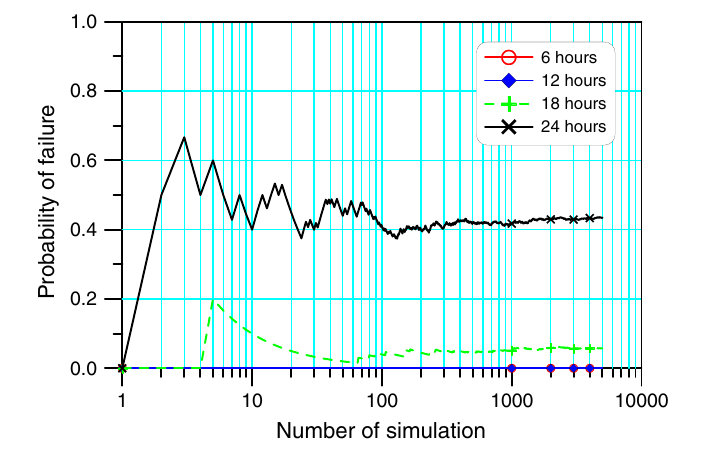
\includegraphics[width=0.48\linewidth]{dados/cho_fig8.png}\\[2pt]{\footnotesize Cho (2014)}\\[4pt]
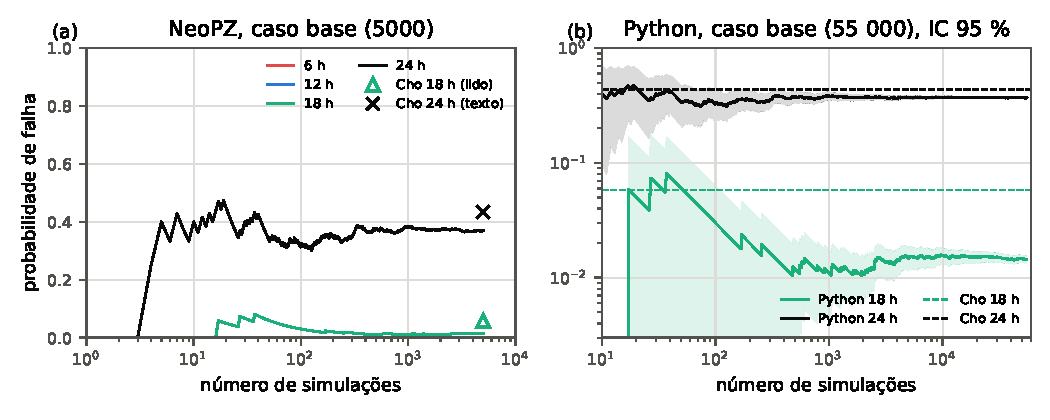
\includegraphics[width=0.9\linewidth]{figs/fig8_conv.pdf}\\{\footnotesize este trabalho}
\caption{A Fig.~8: a $P_f$ no instante contra o número de simulações. (a) NeoPZ, 5000, na ordem das realizações, com os
valores finais de Cho. (b) O Python com 55\,000 realizações e o IC 95\,\% (escala log): em 18~h a $P_f$ converge para
\pfPyBaseDz\,\%, longe dos 5,8\,\% de Cho.}
\label{fig:f8}
\end{figure}

\clearpage
\section{O efeito de CoV e $l_v$: as Figs.~9 e 10}\label{sec:casos}
\begin{itemize}
  \item \textbf{Fig.~9 (Figs.~\ref{fig:f9} e \ref{fig:f9b}):} as curvas acumuladas têm a mesma ordem e forma das de Cho.
    A fração na base cresce com o CoV em 12 e 18~h (com $k_s$ baixo, a água empoça sobre camadas menos permeáveis e a
    frente demora), cai com $l_v$ em 12 e 18~h e cresce com $l_v$ em 24~h. Os nossos valores ficam 5 a 10 pontos acima
    dos de Cho em 12~h; em 18 e 24~h, a até 7 pontos, para os dois lados (Tabela~\ref{tab:alvos}).
  \item \textbf{Fig.~10 em 24~h (Fig.~\ref{fig:f10}b, Tabela~\ref{tab:fig10}):} as tendências de Cho se repetem nos 15
    casos: a $P_f$ cresce com $l_v$ e cai com o CoV (com CoV maior, mais solo tem $k_s < q$ e entra menos água). Os nossos
    valores ficam \difVqMin{} a \difVqMax{} pontos abaixo dos de Cho; a diferença é maior com $l_v$ pequeno
    (6,4 pontos no caso base) e cai a 1--2 pontos com $l_v = 16$, onde os dois encostam no limite de variável aleatória
    (Seção~\ref{sec:limite}).
  \item \textbf{Fig.~10 em 18~h (Fig.~\ref{fig:f10}a):} não reproduz. Ficamos \difDzMin{} a \difDzMax{} pontos abaixo, e as
    tendências se invertem: com CoV 0,5, Cho tem a $P_f$ \emph{crescendo} com $l_v$ (de 5,8 a 11,3\,\%), e nós a temos
    caindo a zero. A Seção~\ref{sec:dezoito} explica por quê.
  \item \textbf{NeoPZ $\times$ Python:} nos 15 casos e nos dois instantes, $|z| \le \zPyMax$ e a maior diferença é de
    \difPyMax{} ponto. Os dois códigos são o mesmo modelo.
\end{itemize}
% gerado por gera_dados.py; nao edite
\begin{table}[htbp]\centering\footnotesize\setlength{\tabcolsep}{3.5pt}
\caption{A Fig.~10: $P_f$ no instante (FS mínimo $< 1$) em 18 e 24~h, em \%. NeoPZ: 5000 realizações, IC~95\,\% de Wilson; Python: as mesmas realizações (55\,000 no caso base); Cho: a figura digitalizada ($\pm 0{,}2$ ponto). $\Delta$: NeoPZ $-$ Cho, em pontos; $t_{eq}$: o instante em que a nossa $P_f$ iguala a de Cho em 18~h.}\label{tab:fig10}
\begin{tabular}{llrrrrrrrrr}\toprule
& & \multicolumn{4}{c}{18 h} & & \multicolumn{4}{c}{24 h} \\\cmidrule{3-6}\cmidrule{8-11}
CoV & $l_v$ (m) & NeoPZ & Python & Cho & $\Delta$ & $t_{eq}$ (h) & NeoPZ [IC 95\,\%] & Python & Cho & $\Delta$ \\\midrule
0{,}5 & 0.5 & 1{,}54 & 1{,}45 & 5{,}8 & \ensuremath{-}4{,}3 & 20{,}1 & 37{,}1 [35{,}8; 38{,}4] & 36{,}9 & 43{,}5 & \ensuremath{-}6{,}4 \\
0{,}5 & 2 & 0{,}10 & 0{,}10 & 8{,}1 & \ensuremath{-}8{,}0 & 20{,}4 & 45{,}9 [44{,}6; 47{,}3] & 46{,}0 & 50{,}1 & \ensuremath{-}4{,}2 \\
0{,}5 & 4 & 0{,}00 & 0{,}00 & 9{,}1 & \ensuremath{-}9{,}1 & 20{,}4 & 48{,}7 [47{,}3; 50{,}1] & 48{,}8 & 52{,}0 & \ensuremath{-}3{,}3 \\
0{,}5 & 8 & 0{,}00 & 0{,}00 & 10{,}3 & \ensuremath{-}10{,}3 & 20{,}5 & 51{,}0 [49{,}6; 52{,}4] & 51{,}1 & 53{,}3 & \ensuremath{-}2{,}3 \\
0{,}5 & 16 & 0{,}00 & 0{,}00 & 11{,}3 & \ensuremath{-}11{,}3 & 20{,}5 & 52{,}4 [51{,}0; 53{,}7] & 52{,}5 & 54{,}3 & \ensuremath{-}1{,}9 \\
\addlinespace
1{,}0 & 0.5 & 6{,}26 & 5{,}94 & 9{,}1 & \ensuremath{-}2{,}8 & 19{,}1 & 24{,}2 [23{,}1; 25{,}4] & 24{,}1 & 27{,}5 & \ensuremath{-}3{,}3 \\
1{,}0 & 2 & 2{,}26 & 2{,}14 & 6{,}2 & \ensuremath{-}3{,}9 & 19{,}1 & 32{,}3 [31{,}0; 33{,}6] & 32{,}3 & 35{,}1 & \ensuremath{-}2{,}8 \\
1{,}0 & 4 & 0{,}68 & 0{,}66 & 5{,}3 & \ensuremath{-}4{,}6 & 19{,}4 & 35{,}1 [33{,}7; 36{,}4] & 35{,}1 & 37{,}1 & \ensuremath{-}2{,}0 \\
1{,}0 & 8 & 0{,}22 & 0{,}18 & 6{,}1 & \ensuremath{-}5{,}9 & 19{,}9 & 37{,}0 [35{,}7; 38{,}4] & 37{,}1 & 39{,}1 & \ensuremath{-}2{,}1 \\
1{,}0 & 16 & 0{,}20 & 0{,}20 & 7{,}0 & \ensuremath{-}6{,}8 & 20{,}1 & 38{,}5 [37{,}2; 39{,}9] & 38{,}6 & 40{,}2 & \ensuremath{-}1{,}7 \\
\addlinespace
1{,}5 & 0.5 & 7{,}94 & 7{,}70 & 10{,}3 & \ensuremath{-}2{,}4 & 19{,}2 & 19{,}4 [18{,}3; 20{,}5] & 19{,}2 & 21{,}8 & \ensuremath{-}2{,}4 \\
1{,}5 & 2 & 3{,}94 & 3{,}84 & 6{,}6 & \ensuremath{-}2{,}7 & 18{,}6 & 26{,}9 [25{,}6; 28{,}1] & 26{,}8 & 28{,}2 & \ensuremath{-}1{,}3 \\
1{,}5 & 4 & 1{,}82 & 1{,}82 & 4{,}9 & \ensuremath{-}3{,}1 & 18{,}7 & 29{,}0 [27{,}8; 30{,}3] & 29{,}0 & 30{,}2 & \ensuremath{-}1{,}2 \\
1{,}5 & 8 & 0{,}80 & 0{,}80 & 4{,}9 & \ensuremath{-}4{,}1 & 19{,}0 & 31{,}0 [29{,}8; 32{,}3] & 31{,}0 & 32{,}1 & \ensuremath{-}1{,}1 \\
1{,}5 & 16 & 0{,}54 & 0{,}54 & 5{,}1 & \ensuremath{-}4{,}6 & 19{,}2 & 32{,}1 [30{,}9; 33{,}4] & 32{,}2 & 33{,}1 & \ensuremath{-}1{,}0 \\
\bottomrule\end{tabular}\end{table}


\begin{figure}[htbp]\centering
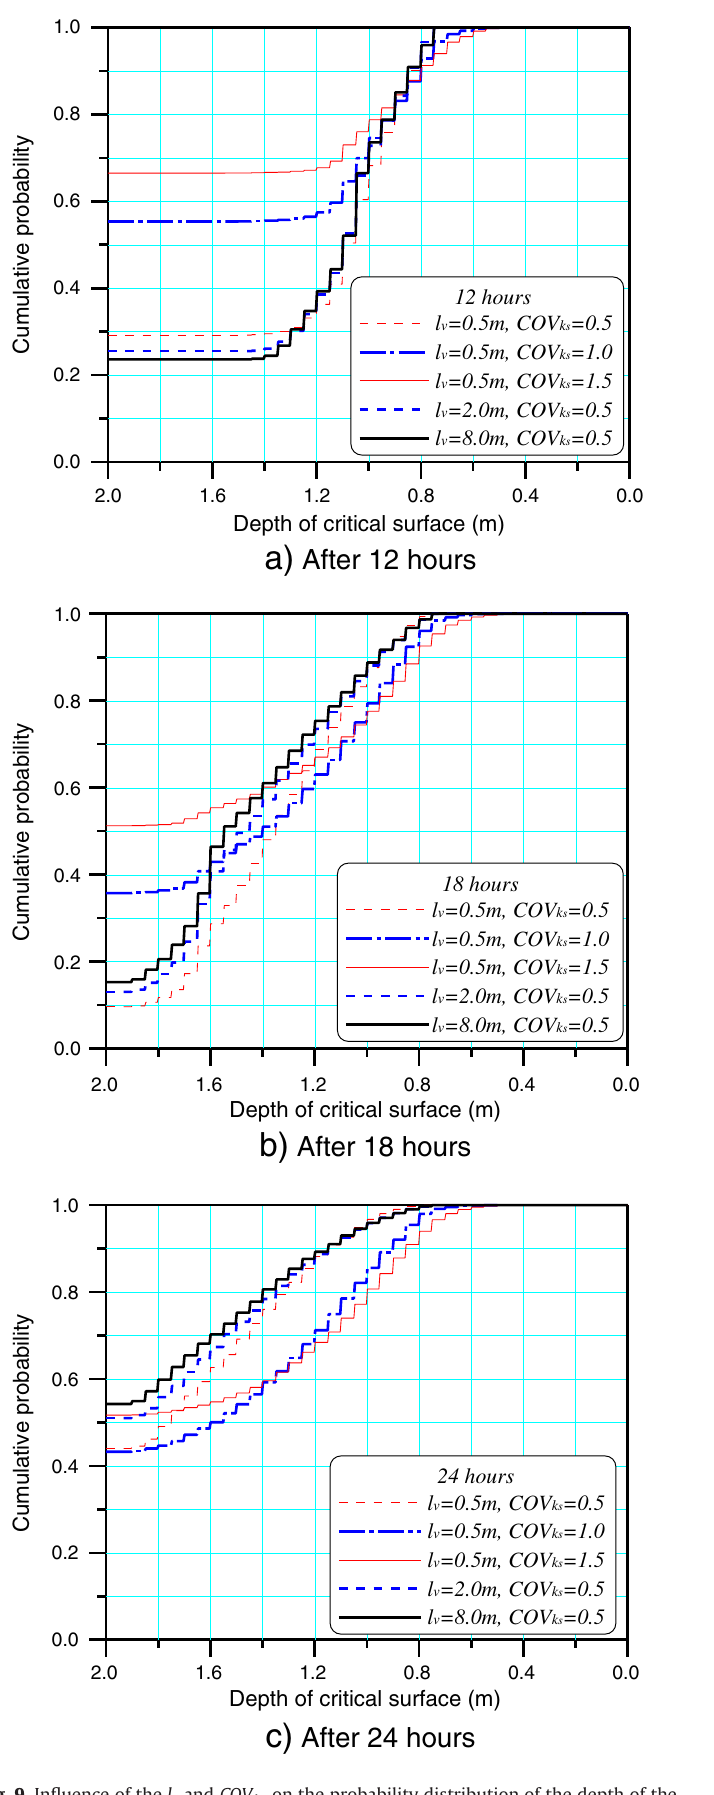
\includegraphics[width=0.40\linewidth]{dados/cho_fig9.png}\\[2pt]{\footnotesize Cho (2014)}\\[4pt]
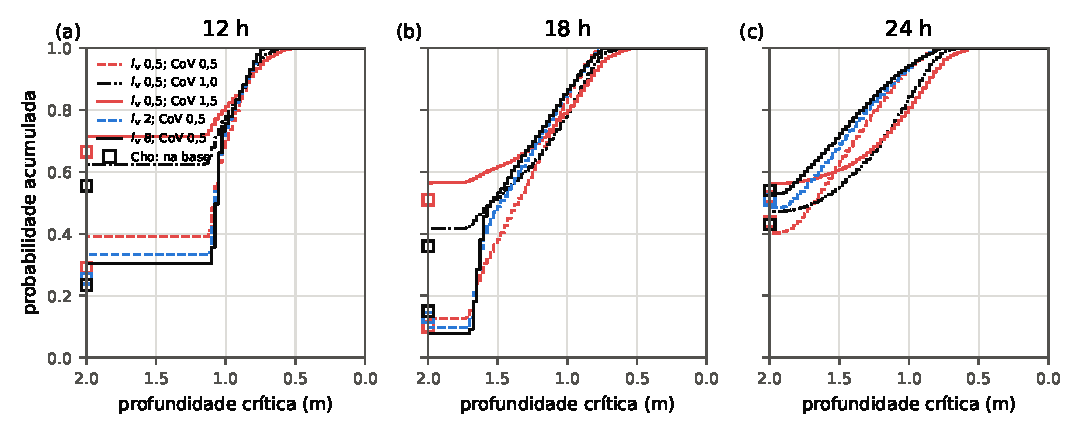
\includegraphics[width=\linewidth]{figs/fig9_cdf.pdf}\\{\footnotesize este trabalho}
\caption{A Fig.~9: $P(z_{crit} \ge d)$ nos cinco casos de Cho em 12, 18 e 24~h (NeoPZ). Os quadrados em 2,0~m são as
frações na base lidas de Cho, na cor de cada caso.}
\label{fig:f9}
\end{figure}

\begin{figure}[htbp]\centering
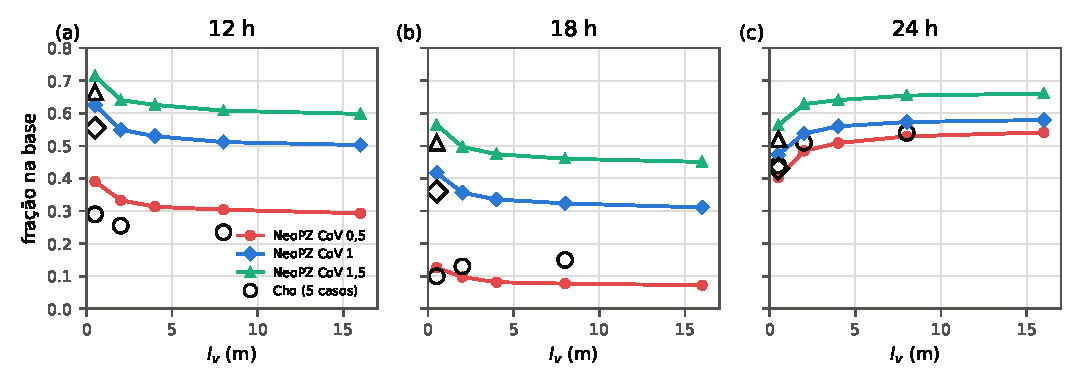
\includegraphics[width=\linewidth]{figs/fig9_base.pdf}
\caption{A fração de superfícies críticas na base nos 15 casos (NeoPZ) contra $l_v$, por CoV; os marcadores vazados
são os cinco casos de Cho (Fig.~9), com o símbolo do CoV.}
\label{fig:f9b}
\end{figure}

\begin{figure}[htbp]\centering
\lado{dados/cho_fig10.png}{0.30}{figs/fig10_pf.pdf}{0.68}
\caption{A Fig.~10: a $P_f$ em 18 e 24~h contra $l_v$. NeoPZ com o IC 95\,\% de Wilson (cheio), Python (+), Cho
(tracejado, vazado) e o limite de variável aleatória ($\star$, em $l_v \to \infty$).}
\label{fig:f10}
\end{figure}

\clearpage
\section{O limite de variável aleatória}\label{sec:limite}
Com $l_v \to \infty$, o campo vira uma variável aleatória: a coluna é homogênea e a $P_f(T) = P(k_s > k^*(T))$, com $k^*$
o $k_s$ que faz o FS mínimo em $T$ valer 1 (bisseção do V3.2, quad ny 80; Fig.~\ref{fig:limite}a).
\begin{itemize}
  \item \textbf{24~h:} $k^* = \kstarVquatro\,q$ e $P = \limVquatroA/\limVquatroB/\limVquatroC$ para CoV 0,5/1,0/1,5. O
    nosso MC com $l_v = 16$ dá \mcDezesseisA/\mcDezesseisB/\mcDezesseisC{} e o de Cho 0,543/0,402/0,331: os dois ficam
    logo abaixo do limite, e a Fig.~10b de Cho ainda sobe com $l_v$. \textbf{Os valores de Cho em 24~h fecham com a
    física.}
  \item \textbf{20~h:} $k^* = \kstarVinte\,q$ e $P = \limVinteA/\limVinteB/\limVinteC$.
  \item \textbf{18~h:} $k^* = \kstarDezoito\,q$ e $P = \limDezoitoA/\limDezoitoB/\limDezoitoC$. Com $l_v = 16$, o nosso MC
    dá \mcDezesseisDezoitoA/\mcDezesseisDezoitoB/\mcDezesseisDezoitoC{}, coerente; Cho dá 0,113/0,070/0,051, de 8 a mais
    de 50 vezes o limite. Numa coluna homogênea a frente só chega à base até 18~h se a zona molhada ficar não saturada,
    e isso exige $k_s \gg q$ (Fig.~\ref{fig:limite}a: o FS de 18~h fica acima de 1,05 até $k_s \approx 5q$).
\end{itemize}
\begin{figure}[htbp]\centering
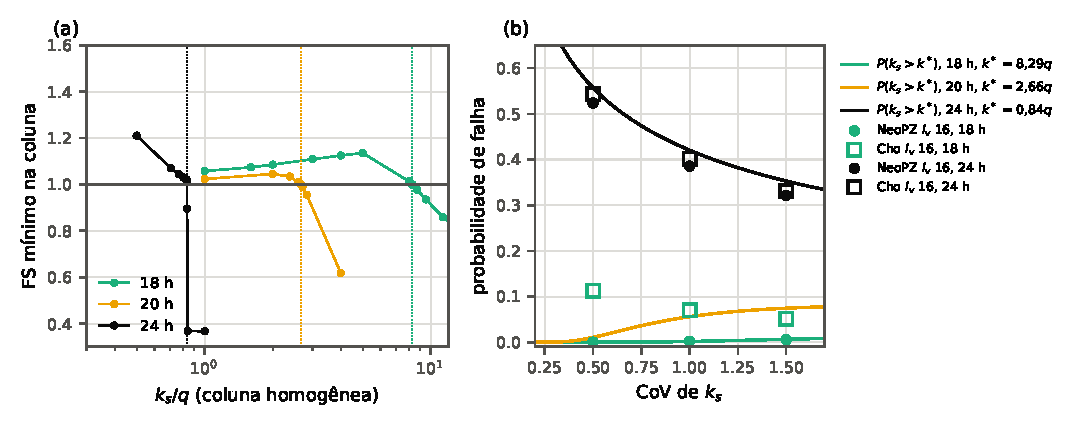
\includegraphics[width=\linewidth]{figs/fig_limite.pdf}
\caption{O limite de variável aleatória. (a) O FS mínimo em 18, 20 e 24~h numa coluna homogênea, contra $k_s/q$ (os
pontos da bisseção do V3.2, quad ny 80; em 18~h também a grade do V3.3, quad ny 200); as verticais são os $k^*$. (b)
$P(k_s > k^*)$ contra o CoV, o nosso MC e o de Cho com $l_v = 16$~m. A grade fina de $k_s$ não existe; o painel (a) usa
só os pontos já rodados.}
\label{fig:limite}
\end{figure}

\section{Por que os 18~h de Cho não se reproduzem}\label{sec:dezoito}
\begin{itemize}
  \item \textbf{O artigo é inconsistente consigo mesmo em 18~h.} Os seus valores de 24~h batem com o limite de variável
    aleatória do próprio modelo (Seção~\ref{sec:limite}); os de 18~h, com $l_v = 16$, ficam muito acima dele. Os 11,3\,\% da
    Fig.~10a com $l_v = 16$ e CoV 0,5 pediriam $k^*(18\,\mathrm{h}) \approx 1{,}6q$, e não há esquema numérico que dê
    isso: nas 20 variantes do V3.3 (tri com massa concentrada e consistente, quad, ny 40 e 200, $\Delta t$ 0,1 e 0,025~h,
    Python na forma mista e na forma em $h$ da Eq.~1 de Cho), $k^*(18\,\mathrm{h})$ fica entre 8,28$q$ e 8,98$q$. Pela regra
    fixada antes do estudo ($k^* \ge 6q$ em todas), o artigo é inconsistente.
  \item \textbf{A tendência se inverte.} Com CoV 0,5, Cho tem $P_f(18\,\mathrm{h})$ crescendo com $l_v$; no nosso modelo,
    quanto maior $l_v$, mais a coluna se parece com a homogênea, que não falha em 18~h.
  \item \textbf{O tempo.} As $P_f$ de Cho em 18~h igualam as nossas entre \tEqMin{} e \tEqMax~h ($t_{eq}$ na
    Tabela~\ref{tab:fig10}; Fig.~\ref{fig:pft}). Com $P_f(t)$ subindo depressa entre 18 e 22~h, um atraso de 1--2~h no
    instante de saída (ou na chegada da frente) mudaria muito os 18~h e pouco os 24~h. É só uma hipótese: o artigo não dá
    o passo nem o esquema.
  \item \textbf{12~h:} Cho tem $P_f = 0$ em todos os casos; nós temos 0 no caso base e até \pfDozeMax\,\% com CoV 1,5. A
    diferença é pequena e vai na mesma direção da fração na base, maior que a de Cho em 12~h.
\end{itemize}
\begin{figure}[htbp]\centering
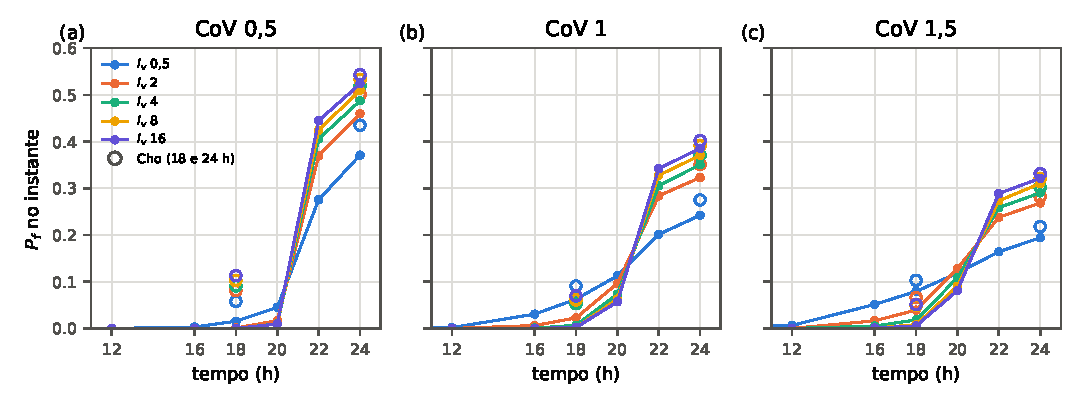
\includegraphics[width=\linewidth]{figs/fig_pf_t.pdf}
\caption{A nossa $P_f$ no instante de 12 a 24~h (NeoPZ, os instantes gravados: 12, 16, 18, 20, 22 e 24~h) e os valores de
Cho em 18 e 24~h (círculos vazados). Os de 18~h caem entre as nossas curvas de 18 e 20~h.}
\label{fig:pft}
\end{figure}

\clearpage
\section{As conferências do método}\label{sec:metodo}
\subsection{NeoPZ, Python, malha, elemento e $\varepsilon$}
\begin{itemize}
  \item \textbf{NeoPZ $\times$ Python:} nos 15 casos, $|z| \le \zPyMax$ (Tabela~\ref{tab:fig10}). Antes da campanha, o V2.2
    pareou as realizações uma a uma (198 de 200 com $|\Delta t_{passagem}| \le 0{,}2$~h, mediana de $|\Delta FS| \le
    0{,}0007$) e o V2.4 conferiu o campo ($\ln k_s$ igual ao do Python até $5\times10^{-10}$).
  \item \textbf{Malha e elemento (Tabela~\ref{tab:estudos}):} com ny 200, triângulos com massa concentrada ou consistente,
    a $P_f$ de 18 e 24~h muda no máximo 2 pares discordantes em 2000. A malha de produção está convergida.
  \item \textbf{$\varepsilon = 10^{-4}$, descartado:} \epsParou{} das \epsN{} realizações (\epsParouPct\,\%) pararam (o
    transiente não convergiu), e \epsCens{} delas sem travessia antes da parada: a falha delas em 24~h não se sabe, e os
    limites da censura vão de \epsLimLo\,\% a \epsLimHi\,\%. Não dá para usar. O estudo no PC (V2.7: 5000 pareadas em
    Python, 650 no NeoPZ) mostrou que $P_f(24\,\mathrm{h})$ cai $1{,}5 \pm 0{,}2$ ponto de $10^{-3}$ para $10^{-4}$; o
    $\varepsilon$ faz parte do modelo (o $k_r$ perto da saturação, que o artigo também não fixa sem ambiguidade: a sua
    Fig.~2b é $\approx 1{,}4$ vez a Eq.~2--2) e fica em $10^{-3}$. Esse 1,5 ponto é uma parte pequena da diferença de 1 a 6
    pontos em 24~h.
\end{itemize}
% gerado por gera_dados.py; nao edite
\begin{table}[htbp]\centering\footnotesize\setlength{\tabcolsep}{3.5pt}
\caption{Os estudos do método (CoV 0,5), pareados com as realizações de mesmo número da produção (quad, ny 80, $\varepsilon = 10^{-3}$). $b/c$: pares discordantes (só o estudo falha / só a produção falha). $P_f$ em \%.}\label{tab:estudos}
\begin{tabular}{lrrrrrrrr}\toprule
estudo & $N$ & paradas & $P_f$ 18 h & produção & $b/c$ & $P_f$ 24 h & produção & $b/c$ \\\midrule
ny 200 ($l_v$ 0,5) & 2\,000 & 0 & 1{,}15 & 1{,}15 & 0/0 & 37{,}2 & 37{,}3 & 0/2 \\
ny 200 ($l_v$ 16) & 2\,000 & 0 & 0{,}00 & 0{,}00 & 0/0 & 53{,}1 & 53{,}0 & 2/0 \\
tri, massa concentrada & 2\,000 & 0 & 1{,}20 & 1{,}15 & 1/0 & 37{,}2 & 37{,}3 & 0/1 \\
tri, massa consistente & 2\,000 & 0 & 1{,}20 & 1{,}15 & 1/0 & 37{,}2 & 37{,}3 & 0/1 \\
$\varepsilon = 10^{-4}$ (descartado) & 5\,000 & 1\,506 & 1{,}67 & 1{,}78 & 0/4 & 41{,}4 & 42{,}6 & 0/43 \\
\bottomrule\end{tabular}\end{table}


\subsection{Line sampling}\label{sec:ls}
O line sampling (LS) roda no caso base, com $M = 100$ e o NeoPZ quad ny 80, na direção da média dos $\xi$ das falhas
de um piloto de MC (Tabela~\ref{tab:ls}, Fig.~\ref{fig:ls}).
\begin{itemize}
  \item \textbf{A direção decide o custo.} O piloto de 5000 sem truncar dá CoV por linha de \lsCvRec{} (\lsCvRecCem{} nas
    mesmas 100 linhas do T1); truncado nos modos 0--9 (T1), \lsCvTdez{}, cerca de metade das análises. O LS em estágios
    (T2: direção reestimada das linhas de um piloto ruim de 500, semente nova) dá \lsCvEst; o piloto de 500 sozinho,
    \lsCvPqui{}.
  \item \textbf{18~h:} todos os LS ficam um pouco acima do MC. T1 e T2 têm sementes independentes; juntos dão
    \lsPool\,\% (EP \lsPoolSE), $z = \zPool$ contra o Python de 55\,000 (\pfPyBaseDz\,\%). A explicação é a diferença de
    modelo na cauda: nos \nRaizes{} pontos de raiz das linhas que mais pesam, o FS do C++ fica \dfsRaiz{}$\times10^{-3}$
    (EP \dfsRaizSE$\times10^{-3}$) abaixo do Python (Fig.~\ref{fig:ls}c). Deslocar o FS do MC em Python por esse valor
    aumenta a $P_f(18\,\mathrm{h})$ em \deslocRaiz{} ponto (0,12 a 0,16 para um desvio de 0,003 a 0,004; Fig.~\ref{fig:ls}d),
    para \pyCorr\,\%; contra esse valor, $z = \zPoolCorr$. O MC do próprio NeoPZ (\pfBaseDz\,\%) já fica acima do Python
    na mesma direção.
  \item \textbf{24~h:} o FS cai num penhasco até o patamar da coluna cheia, e a secante aceitava raízes não localizadas
    (\lsVq\,\%, $z = \zVq$). A \texttt{busca=cerca} (aceita só com um ponto seguro e um em falha a menos de 0,01 em $c$)
    corrige isso: \lsVqC\,\% com \lsAnVqC{} análises por linha, igual às raízes corrigidas pelo $t_{passagem}$ (34,8\,\%),
    $z = \zVqC$ contra o MC em Python de 5000.
  \item \textbf{Segunda raiz:} as 16 linhas que mais pesam, varridas de $c_i - 2$ a $c_i + 4$, cruzam FS $= 1$ uma só
    vez; só uma tem um ondulado de $10^{-4}$ no FS perto da raiz, sem nova travessia. Não há segunda região de falha.
\end{itemize}
% gerado por gera_dados.py; nao edite
\begin{table}[htbp]\centering\footnotesize\setlength{\tabcolsep}{4pt}
\caption{O line sampling no caso base (CoV 0,5; $l_v$ 0,5~m), $M = 100$, NeoPZ quad ny 80. $z$: contra o MC em Python de 55\,000 ($P_f(18\,\mathrm{h}) = 1{,}45\,\%$). CoV por linha: o desvio de $p$ entre as linhas sobre a média.}\label{tab:ls}
\begin{tabular}{llrrrrrr}\toprule
direção & semente & linhas & $P_f$ (\%) & CoV (\%) & CoV por linha & análises/linha & $z$ \\\midrule
\multicolumn{8}{l}{\emph{18 h}} \\
piloto p5000, sem truncar & 7 & 200 & 1{,}81 & 11{,}7 & 1{,}65 & 4{,}00 & +1{,}63 \\
o mesmo, linhas 0--99 & 7 & 100 & 1{,}73 & 14{,}7 & 1{,}47 & 3{,}96 & +1{,}06 \\
piloto p500 (6 falhas) & 7 & 200 & 1{,}82 & 29{,}0 & 4{,}10 & 5{,}02 & +0{,}69 \\
T1: p5000 truncado 0--9 & 7 & 100 & 1{,}68 & 10{,}3 & 1{,}03 & 3{,}89 & +1{,}27 \\
T1: p5000 truncado 0--4 & 7 & 100 & 1{,}71 & 10{,}9 & 1{,}09 & 3{,}79 & +1{,}33 \\
T2: estágio 2 (direção das linhas) & 9 & 100 & 2{,}18 & 12{,}2 & 1{,}22 & 3{,}75 & +2{,}69 \\
T1 0--9 + T2 (inverso da variância) & & 200 & 1{,}83 & 7{,}9 & & & +2{,}46 \\
\multicolumn{8}{l}{\emph{24 h} ($z$ contra o MC em Python de 5000, $37{,}14\,\%$)} \\
piloto p5000, secante & 7 & 48 & 35{,}75 & 4{,}8 & 0{,}33 & 7{,}92 & \ensuremath{-}0{,}76 \\
piloto p5000, \texttt{busca=cerca} & 7 & 48 & 34{,}82 & 4{,}7 & 0{,}33 & 9{,}08 & \ensuremath{-}1{,}30 \\
\bottomrule\end{tabular}\end{table}

\begin{figure}[htbp]\centering
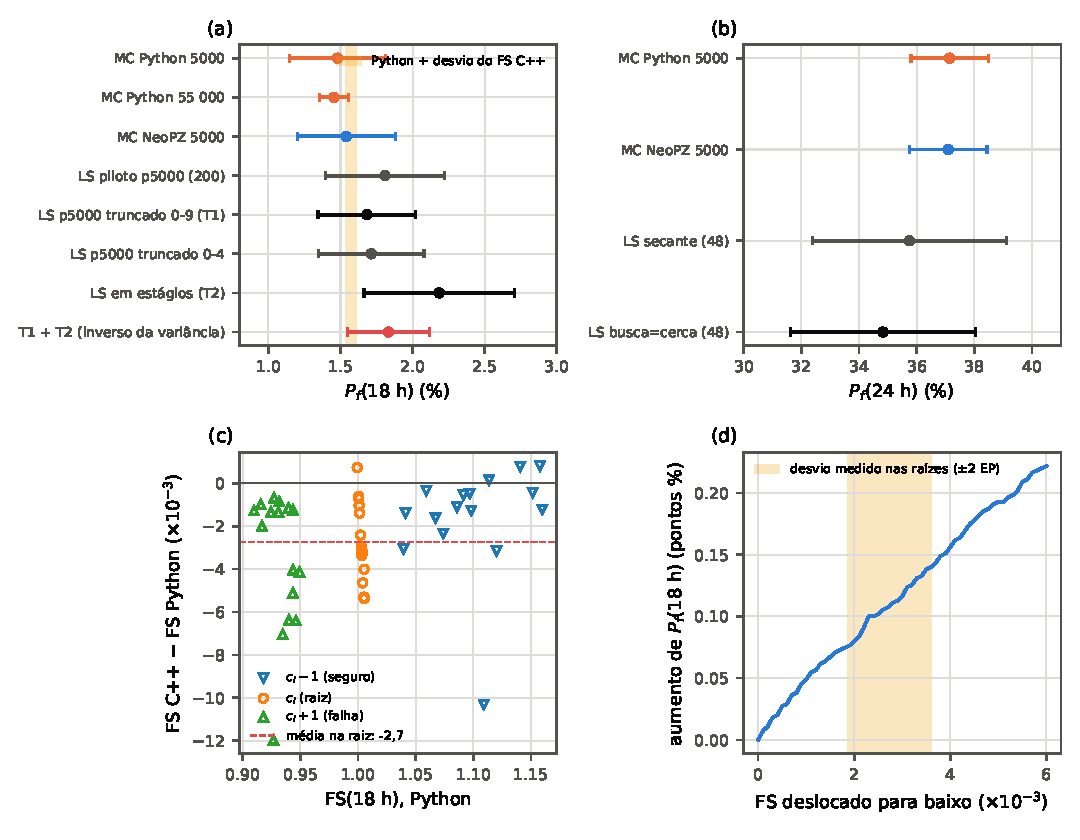
\includegraphics[width=\linewidth]{figs/fig_ls.pdf}
\caption{O line sampling no caso base. (a) $P_f(18\,\mathrm{h})$ com o IC 95\,\%: os MC, os LS e a faixa do MC em
Python deslocado pelo desvio de FS do C++ (0,002 a 0,004). (b) $P_f(24\,\mathrm{h})$: a secante e a \texttt{busca=cerca}.
(c) FS C++ $-$ FS Python nos pontos de raiz das 16 linhas e a $\pm 1$ em $c$. (d) O aumento da $P_f(18\,\mathrm{h})$ do MC
em Python (55\,000) quando o FS é deslocado para baixo.}
\label{fig:ls}
\end{figure}

\section{Conclusões}
\begin{itemize}
  \item \textbf{Reproduz:} a Fig.~3 (FS e frentes dentro das leituras), as formas das Figs.~5 a 9 (o histograma de
    $z_{crit}$, o FS bimodal de 24~h, as medianas), o limite de variável aleatória e a Fig.~10 em 24~h, com todas as
    tendências e a $P_f$ \difVqMin{} a \difVqMax{} pontos abaixo de Cho.
  \item \textbf{Não reproduz:} a Fig.~10 em 18~h. Os valores do artigo com $l_v$ grande contradizem o limite de variável
    aleatória do próprio modelo, e nenhum esquema dos 20 testados aproxima o buraco. Os 18~h de Cho não servem de alvo.
  \item \textbf{O método está conferido:} NeoPZ = Python nos 15 casos, a malha e o elemento convergidos, o $\varepsilon$
    fixado (e o estudo de $10^{-4}$ no fermi descartado pelas paradas), o LS de acordo com o MC, com o excesso de 18~h
    explicado pelo FS C++ $\approx 0{,}003$ abaixo do Python nas raízes.
  \item \textbf{O que falta:} as figuras de Cho sem números (Figs.~5, 7 e 9 só têm a base e as modas lidas); o gráfico
    fino FS$(k_s)$ do limite usa só os pontos da bisseção, porque não houve rodada nova para este relatório.
\end{itemize}

\begin{thebibliography}{9}
\bibitem{cho2014} S.~E.~Cho. Probabilistic stability analysis of rainfall-induced landslides considering spatial
  variability of permeability. \emph{Engineering Geology}, 171:11--20, 2014. doi:10.1016/j.enggeo.2013.12.015.
\bibitem{notas} Cho (2014): talude infinito 1D com campo de $k_s$ sob chuva, extração para reprodução. Notas de leitura,
  \path{research_notes/Reprodução dos artigos novos/cho2014.md}, 23/11/2026.
\bibitem{wilson1927} E.~B.~Wilson. Probable inference, the law of succession, and statistical inference.
  \emph{Journal of the American Statistical Association}, 22(158):209--212, 1927.
\bibitem{koutsourelakis2004} P.~S.~Koutsourelakis, H.~J.~Pradlwarter, G.~I.~Schuëller. Reliability of structures in
  high dimensions, part~I: algorithms and applications. \emph{Probabilistic Engineering Mechanics}, 19(4):409--417, 2004.
\end{thebibliography}

\appendix
\section{Arquivos e como refazer}\label{sec:arquivos}
\begin{itemize}
  \item \textbf{A campanha:} \path{Projects/SlopeRandomFieldRefinement/cluster/cho2014_casos.sbatch} com
    \path{casos_cho2014.txt}; baixada em \path{~/projects/runs/fermi_cho2014}; o resumo é o \texttt{resumo\_cho2014.py}
    (saída em \path{dados/resultado.txt} e \path{dados/resumo.json}).
  \item \textbf{A referência em Python:} \path{~/projects/runs/cho2014_python} (\texttt{coluna\_ref.py}, resumo
    \texttt{referencias\_1d/resumo\_ref.py}).
  \item \textbf{Os estudos:} \path{~/projects/runs/coluna_estudos} (V2.2--V2.7, V3.2 e V3.3; \texttt{LEIAME.md}); o
    determinístico da Fig.~3 é o \texttt{q80} de \path{~/projects/runs/coluna_verificacao_independente/det} (quad ny 80);
    o Python de \path{cho2014_python/det}.
  \item \textbf{O line sampling:} \path{~/projects/runs/coluna_ls_piloto} (\texttt{LEIAME.md}, \texttt{LEIAME\_adaptativo.md}
    com a revisão, \path{ls_p5000_T24_cerca/}, \path{segunda_raiz/} com \path{py_raizes/}).
  \item \textbf{Este relatório:} \texttt{gera.sh} refaz o resumo, roda o \texttt{gera\_dados.py} (tabelas em \path{tab/},
    números em \path{numeros.tex}, figuras em \path{figs/}, recortes das figuras de Cho em \path{dados/}) e o \LaTeX.
    Nenhuma simulação é rodada.
\end{itemize}
\end{document}
